\section{Dirac and narrow-gap materials}\label{sec:7.3}

The pentatelluride ZrTe$_5$ has a band gap of about \SI{24}{meV}, and near the gap its electrons move at about $10^{-3}$ of the speed of light whatever their energy. Dark matter of about \SI{8}{keV} can carry an electron across this gap, about forty times lighter than the \SI{0.333}{MeV} that silicon requires (\cref{sec:1.3}). Materials of this kind are called Dirac materials, because near the gap the electrons obey the Dirac equation of a relativistic particle, with a velocity $v_{\mathrm{D}}$ in place of the speed of light and half the gap in place of the mass. They were proposed as targets for sub-MeV dark matter~\cite{hochberg2018detection}. As in the superconductor of \cref{sec:7.2}, the cheapest excitation is a pair whose energy starts at twice a half-gap, here an electron and a hole on either side of a band gap. Pairs are cheap in momentum too: the bands are linear, and slow enough, $v_{\mathrm{D}} < v_{\mathrm{max}}$, for a dark-matter particle to outrun them. And the same electrons screen the interaction in a way that is fixed by two numbers, $v_{\mathrm{D}}$ and the dielectric constant of everything else in the crystal.

\subsection{The Dirac Hamiltonian from \texorpdfstring{$\vect{k}\cdot\vect{p}$}{k.p} theory}

The $\vect{k}\cdot\vect{p}$ expansion of \cref{sec:3.3} assumed a band well separated from all others. Near a point where two bands nearly touch, the second-order formula \cref{eq:3.3-mass} breaks down, because its energy denominator becomes small, and the two bands have to be treated together. Take a time-reversal-invariant momentum $\vect{k}_0$, such as $\mathrm{\Gamma}$, in a crystal with inversion symmetry. Time reversal combined with inversion maps a Bloch state at $\vect{k}$ onto a different state at the same $\vect{k}$, and because time reversal squares to $-1$ for electrons, every band is then doubly degenerate at every $\vect{k}$: the Kramers degeneracy. Suppose that at $\vect{k}_0$ two such doublets lie close to each other and far from all other bands: a conduction doublet at energy $+\Delta_{\mathrm{D}}$ and a valence doublet at $-\Delta_{\mathrm{D}}$, measured from the middle of the gap, with opposite parity under inversion. We write $\Delta_{\mathrm{D}}$ for this \emph{half-gap}. Keep these four states exactly and drop the remote bands. At first order in $\delta\vect{k} = \vect{k} - \vect{k}_0$, the Bloch Hamiltonian of \cref{sec:3.3} acts in the four-state space through the matrix elements of $\delta\vect{k}\cdot\vect{v}$, with $\vect{v}$ the velocity operator of \cref{eq:3.2-dHk}. The velocity is odd under inversion, and its matrix elements between two states of the same parity vanish. Only the block between the doublets survives:
\begin{equation}
  H_{\vect{k}_0+\delta\vect{k}} = \begin{pmatrix} \Delta_{\mathrm{D}}\,\mathbb{1} & M(\delta\vect{k}) \\ M(\delta\vect{k})^\dagger & -\Delta_{\mathrm{D}}\,\mathbb{1} \end{pmatrix} , \qquad M(\delta\vect{k}) = \sum_{i=1}^{3}\delta k_iM_i ,
  \label{eq:7.3-block}
\end{equation}
where $\mathbb{1}$ is the $2\times2$ unit matrix and $M_i$ is the $2\times2$ matrix of the velocity component $v^i$ between the conduction and the valence doublet. The free-electron term $\delta k^2/2m_e$ and the second-order couplings to the remote bands are of order $\delta k^2$; they bend the bands at large $\delta k$, and we return to them when we fix the cutoff.

The block $M(\delta\vect{k})$ is not arbitrary, and the Kramers degeneracy is what pins it down. Square \cref{eq:7.3-block}. The off-diagonal blocks of $H^2$ are $\Delta_{\mathrm{D}}M - M\Delta_{\mathrm{D}}$, which cancel because $\Delta_{\mathrm{D}}$ multiplies the unit matrix, and $H^2$ is block diagonal, with the blocks $\Delta_{\mathrm{D}}^2 + MM^\dagger$ and $\Delta_{\mathrm{D}}^2 + M^\dagger M$. The eigenvalues of $H$ come in pairs $\pm E$. If each is doubly degenerate at every $\delta\vect{k}$, as the Kramers degeneracy requires, then $E^2$ is a fourfold eigenvalue of $H^2$, and the $2\times2$ matrix $MM^\dagger$ must be a multiple of the unit matrix for every direction of $\delta\vect{k}$. This is a strong condition on the three matrices $M_i$. A general complex $2\times2$ matrix is a combination of the unit matrix and the three Pauli matrices, with eight real coefficients. The Pauli matrices here act within a doublet, not on the electron spin of \cref{eq:7.1-se}, and we write them $\sigma^{\mathrm{d}}_i$, with d for doublet. \Cref{app:D.22} shows step by step what the condition leaves. Up to a common unitary factor, which a choice of basis in the valence doublet absorbs, each $M_i$ is a real combination of the four matrices $\mathbb{1}$, $\ii\sigma^{\mathrm{d}}_1$, $\ii\sigma^{\mathrm{d}}_2$ and $\ii\sigma^{\mathrm{d}}_3$: four real numbers per direction instead of eight. A unitary change of basis within each doublet turns these three four-vectors rigidly, by any rotation of four-dimensional space, and a suitable rotation brings $M$ to the form $M = \sum_iv_i\,\delta k_i\,\sigma^{\mathrm{d}}_i$ with three real velocities $v_i$ along three principal axes. In that basis we define the $4\times4$ Dirac matrices
\begin{equation*}
  \alpha_{\mathrm{D}}^i = \begin{pmatrix} 0 & \sigma^{\mathrm{d}}_i \\ \sigma^{\mathrm{d}}_i & 0 \end{pmatrix} , \qquad \beta_{\mathrm{D}} = \begin{pmatrix} \mathbb{1} & 0 \\ 0 & -\mathbb{1} \end{pmatrix} ,
\end{equation*}
the matrices of \cref{app:C.15} with the subscript D that keeps them apart from the fine-structure constant and the inverse temperature. They anticommute pairwise and square to one. The four-state Hamiltonian then takes the Dirac form.
\begin{keyresult}[Dirac Hamiltonian]
Near a time-reversal-invariant momentum $\vect{k}_0$ of a crystal with inversion symmetry, two Kramers doublets of opposite parity at $\pm\Delta_{\mathrm{D}}$ are described, to first order in $\delta\vect{k} = \vect{k} - \vect{k}_0$, by
\begin{equation}
  H_{\vect{k}_0+\delta\vect{k}} = \sum_{i=1}^{3}v_i\,\delta k_i\,\alpha_{\mathrm{D}}^i + \Delta_{\mathrm{D}}\,\beta_{\mathrm{D}} , \qquad
  \varepsilon_{\pm,\delta\vect{k}} = \pm\Bigl(\sum_iv_i^2\delta k_i^2 + \Delta_{\mathrm{D}}^2\Bigr)^{1/2} ,
  \label{eq:7.3-H}
\end{equation}
with each band doubly degenerate. The velocities $v_i$ are the singular values of the interband velocity matrix elements, and $\Delta_{\mathrm{D}}$ is half the energy separation of the two doublets at $\vect{k}_0$.
\end{keyresult}
\Cref{eq:7.3-H} is the Dirac Hamiltonian of a particle of mass $\Delta_{\mathrm{D}}$, with the speed of light replaced by $v_i$ along the principal axis $i$; it is the form used for ZrTe$_5$ in Refs.~\cite[Eq.~(1.1)]{geilhufe2020dirac} and~\cite{hochberg2018detection}. When the crystal symmetry makes the three velocities equal, $v_i = v_{\mathrm{D}}$, the \emph{Dirac velocity}, and $H = v_{\mathrm{D}}\boldsymbol{\alpha}_{\mathrm{D}}\cdot\delta\vect{k} + \Delta_{\mathrm{D}}\beta_{\mathrm{D}}$ with $E_{\vect{k}} = (v_{\mathrm{D}}^2\delta k^2 + \Delta_{\mathrm{D}}^2)^{1/2}$, the notation of \cref{app:D.22}. The literature usually writes $v_{\mathrm{F}}$ for the Dirac velocity; in this book $v_{\mathrm{F}}$ is the Fermi velocity of the electron gas. One of the $v_i$ may come out negative in the last rotation (\cref{app:D.22}). Its sign does not enter the spectrum or anything else in this section, which depends on $v_i^2$, and we take all three positive.

The two-level Kane model of \cref{sec:3.3} is the same physics in a familiar setting. There the conduction state of GaAs couples to the valence state $|X\rangle$ through $\delta k_xv^x_{cX}$ across the gap $\Eg$, and the two levels repel as $\pm[(\Eg/2)^2 + |v^x_{cX}|^2\delta k_x^2]^{1/2}$, which is \cref{eq:7.3-H} with $\Delta_{\mathrm{D}} = \Eg/2$ and $v_{\mathrm{D}} = |v^x_{cX}|$. Near its bottom the band is parabolic, with mass $\Delta_{\mathrm{D}}/v_{\mathrm{D}}^2 = m_e\Eg/E_P$: the Kane mass \cref{eq:3.3-kane2} without the free-electron term. With $E_P = \SI{22.9}{eV}$ ($|v^x_{cX}| = 4.7\times10^{-3}$) and the GaAs gap of \SI{1.52}{eV}, this is $0.066\,m_e$, within \SI{2}{\percent} of the measured $0.067\,m_e$. A narrow-gap semiconductor is thus a massive Dirac material, and since the Kane energy changes little from one III--V compound to the next, its Dirac velocity stays near $4.7\times10^{-3}$ as the gap closes. That is $1.8\,v_{\mathrm{max}}$, and we will see below that this is too fast for dark-matter scattering.

At $\Delta_{\mathrm{D}} = 0$ the conduction and valence doublets are degenerate at $\vect{k}_0$, and \cref{eq:7.3-H} separates. In the basis of the sums and differences of the conduction and valence states, it becomes two $2\times2$ blocks, $\pm\sum_iv_i\,\delta k_i\,\sigma^{\mathrm{d}}_i$. Each block is a \emph{Weyl node}, a crossing of two nondegenerate bands that uses all three Pauli matrices, so that no small perturbation of the block alone can open a gap. The two nodes have opposite chirality, the sign in front of the block, and only a perturbation that couples them, such as the mass term $\Delta_{\mathrm{D}}\beta_{\mathrm{D}}$, gaps the spectrum. A crystal in which the nodes sit at the same momentum and symmetry keeps $\Delta_{\mathrm{D}} = 0$ is a Dirac semimetal. Na$_3$Bi and Cd$_3$As$_2$ are examples, although their nodes sit on a rotation axis away from the time-reversal-invariant momenta, where a crystal rotation protects them. If inversion or time reversal is broken, the Kramers degeneracy is lifted, the nodes can move apart in momentum, and the material is a Weyl semimetal~\cite{armitage2018weyl}. The sign of $\Delta_{\mathrm{D}}$ distinguishes an ordinary from an inverted band order, and pressure, strain or composition can tune it through zero. ZrTe$_5$ sits close to this transition, which is why its gap is small and why first-principles values disagree on its size: they range from 24 to \SI{35}{meV}~\cite[Table~1]{geilhufe2020dirac} and~\cite[Table~1]{hochberg2018detection}, and the gap is sensitive to the lattice constant used.

The linear form \cref{eq:7.3-H} holds while the neglected terms of order $\delta k^2$ are small compared with $v_i\delta k_i$. Beyond some momentum the bands bend away, and the states there behave like those of an ordinary insulator. We model this by a hard \emph{momentum cutoff} $\Lambda_{\mathrm{D}}$ on $|\delta\vect{k}|$, inside which the Dirac form is used and outside which the states are counted with the remote bands. The value of $\Lambda_{\mathrm{D}}$ is read off a computed band structure, as the momentum at which the bands deviate from linear; for ZrTe$_5$ it is 0.1 to \SI{0.23}{\angstrom^{-1}} depending on the direction, or 200 to \SI{450}{eV}. Finally, let $g_{\mathrm{deg}}$ count the degenerate states per band and wavevector, summed over all Dirac points in the zone: $g_{\mathrm{deg}} = 2$ for one four-component cone, and twice the number of cones in general.

\subsection{Density of states}

How many states does a Dirac cone offer at energy $E$? For the isotropic cone the number of states per volume in one band with energy below $E$ is $g_{\mathrm{deg}}$ times the volume of a sphere of radius $\delta k = (E^2 - \Delta_{\mathrm{D}}^2)^{1/2}/v_{\mathrm{D}}$, divided by $(2\pi)^3$. Differentiating with $\delta k\,\dd(\delta k) = E\,\dd E/v_{\mathrm{D}}^2$ gives the density of states per volume of the conduction band,
\begin{equation}
  \mathcal{N}_{\mathrm{D}}(E) = \frac{g_{\mathrm{deg}}\delta k^2}{2\pi^2}\frac{\dd(\delta k)}{\dd E} = \frac{g_{\mathrm{deg}}}{2\pi^2v_{\mathrm{D}}^3}\,E\,(E^2 - \Delta_{\mathrm{D}}^2)^{1/2}\,\Theta(E - \Delta_{\mathrm{D}}) ,
  \label{eq:7.3-dos}
\end{equation}
and the valence band mirrors it at $-E$. For an anisotropic cone, the substitution $\delta k_i \to \delta k_i v_{\mathrm{D}}/v_i$ shows that $v_{\mathrm{D}}^3$ is replaced by $v_1v_2v_3$. Just above the edge, $E - \Delta_{\mathrm{D}} \ll \Delta_{\mathrm{D}}$, the band is parabolic with mass $\Delta_{\mathrm{D}}/v_{\mathrm{D}}^2$ and $\mathcal{N}_{\mathrm{D}}$ grows as $(E - \Delta_{\mathrm{D}})^{1/2}$, as at any band edge. Far above it, or at any energy in a gapless cone, $\mathcal{N}_{\mathrm{D}} = g_{\mathrm{deg}}E^2/(2\pi^2v_{\mathrm{D}}^3)$, the density of states of massless particles, which vanishes at the node.

The vanishing density of states at $E = 0$ means that an undoped gapless cone has no Fermi surface. Thomas--Fermi screening (\cref{eq:4.4-TF}), which needs a finite density of states at the Fermi level, is then absent, and whatever screening the Dirac electrons provide comes from interband pairs, which we compute below. The factor $1/v_{\mathrm{D}}^3$ means that slow cones have many states: at fixed $E$, halving the velocity multiplies the states by eight. The thermal carriers follow from the parabolic edge. The symmetry of the two bands puts the chemical potential in the middle of the gap. The conduction-electron density is then the intrinsic density \cref{eq:3.3-ni} with both density-of-states masses equal to $\Delta_{\mathrm{D}}/v_{\mathrm{D}}^2$, the spin factor 2 replaced by $g_{\mathrm{deg}}$ and $\Eg = 2\Delta_{\mathrm{D}}$:
\begin{equation}
  \nd_{\mathrm{i}} = g_{\mathrm{deg}}\Bigl(\frac{\Delta_{\mathrm{D}}T}{2\pi v_{\mathrm{D}}^2}\Bigr)^{3/2}\ee^{-\Delta_{\mathrm{D}}/T} , \qquad T \ll \Delta_{\mathrm{D}} .
  \label{eq:7.3-nc}
\end{equation}
For the ZrTe$_5$-like cone of \cref{we:7-zrte5}, with $\Delta_{\mathrm{D}} = \SI{11.8}{meV}$, $v_{\mathrm{D}} = 7.9\times10^{-4}$ and $g_{\mathrm{deg}} = 2$, the edge mass is $0.037\,m_e$. At room temperature $\Delta_{\mathrm{D}}/T = 0.46$ and the material is full of carriers. At \SI{4}{K}, $\Delta_{\mathrm{D}}/T = 34$ and \cref{eq:7.3-nc} gives $\nd_{\mathrm{i}} \approx \SI{0.4}{cm^{-3}}$, within \SI{5}{\percent} of the exact integral over \cref{eq:7.3-dos}; at the millikelvin temperatures of a phonon or charge readout the thermal population is zero for all purposes. A gap of tens of meV is the right size: small enough for light dark matter, large enough to freeze out the carriers.

\subsection{Interband pair threshold}

At $T = 0$, with the chemical potential in the gap, the lower band is full and the upper band empty. The excitations are pairs: an electron at $\vect{k} + \vect{q}$ in the upper band and a hole at $\vect{k}$ in the lower one, with energy $\omega = E_{\vect{k}} + E_{\vect{k}+\vect{q}}$. For given $\vect{q}$, the cheapest pair has $\vect{k} = -\vect{q}/2$. The reason is that $E_{\vect{k}}$ is even and convex in $\vect{k}$, so that $E_{\vect{k}} + E_{\vect{k}+\vect{q}} = E_{-\vect{k}} + E_{\vect{k}+\vect{q}} \ge 2E_{\vect{q}/2}$, with equality at $\vect{k} = -\vect{q}/2$. The pair continuum is therefore
\begin{equation}
  \omega \ge (v_{\mathrm{D}}^2q^2 + 4\Delta_{\mathrm{D}}^2)^{1/2} ,
  \label{eq:7.3-edge}
\end{equation}
the shaded region of \cref{fig:7-dirac}b. The edge is the dispersion of a relativistic particle of mass $2\Delta_{\mathrm{D}}$ and momentum $q$, with $v_{\mathrm{D}}$ in place of the speed of light. In a gapless cone the edge is the line $\omega = v_{\mathrm{D}}q$. Compare the electron gas of \cref{sec:4.5}, whose continuum reaches down to $\omega = 0$ at every $q < 2k_{\mathrm{F}}$: pairs in a Fermi sea can be made at no energy cost, while in a Dirac cone every pair costs at least $v_{\mathrm{D}}q$.

\begin{figure}[tbp]
  \centering
  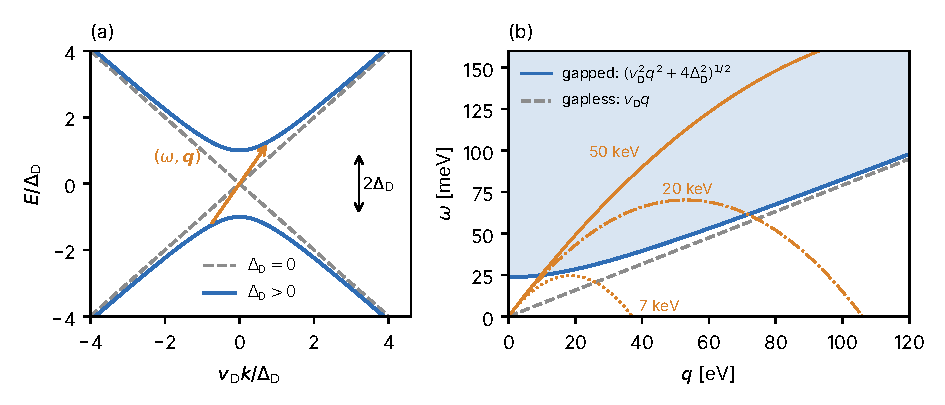
\includegraphics[width=\linewidth]{figures/ch07/fig7_3.pdf}
  \caption{Dirac cones and their pairs. (a) Bands $\pm(v_{\mathrm{D}}^2k^2 + \Delta_{\mathrm{D}}^2)^{1/2}$ of a gapped cone (solid) and of a gapless one (dashed), in units of the half-gap $\Delta_{\mathrm{D}}$; the arrow is an interband pair with energy $\omega$ and momentum $\vect{q}$. (b) Energy $\omega$ against momentum $q$ of the pairs of an isotropic cone with the ZrTe$_5$-like parameters $v_{\mathrm{D}} = 7.9\times10^{-4}$ (geometric mean of the three principal velocities) and $\Delta_{\mathrm{D}} = \SI{11.8}{meV}$ of Ref.~\cite[Table~1 and text below it]{geilhufe2020dirac}. Shaded: the pair continuum $\omega \ge (v_{\mathrm{D}}^2q^2 + 4\Delta_{\mathrm{D}}^2)^{1/2}$; dashed: its edge $\omega = v_{\mathrm{D}}q$ for $\Delta_{\mathrm{D}} = 0$. Orange: the largest energy that dark matter of mass 7, 20 and \SI{50}{keV} can deposit at momentum $q$, $\omega = qv_{\mathrm{max}} - q^2/2m_\chi$ with $v_{\mathrm{max}} = 2.650\times10^{-3}$. The \SI{7}{keV} curve stays just below the continuum; the threshold mass is \SI{8.0}{keV}.}
  \label{fig:7-dirac}
\end{figure}

Dark matter of mass $m_\chi$ can deposit at most $\omega = qv_{\mathrm{max}} - q^2/2m_\chi$ at momentum $q$ (\cref{eq:1.3-region}), and a pair is kinematically allowed where this curve enters the continuum. \Cref{fig:7-dirac}b shows that the velocity decides whether a cone can be reached at all, and the gap decides at which mass. The dark-matter curve lies below the line $\omega = v_{\mathrm{max}}q$, and the continuum edge lies above the line $\omega = v_{\mathrm{D}}q$, so that a cone with $v_{\mathrm{D}} > v_{\mathrm{max}}$ is out of reach of scattering at any mass, with or without a gap. This rules out the III--V narrow-gap semiconductors, with $v_{\mathrm{D}} \approx 1.8\,v_{\mathrm{max}}$, as scattering targets (absorption at $q \approx 0$ is another matter), and it is why the slow cones of ZrTe$_5$, at $v_{\mathrm{D}} = 0.30\,v_{\mathrm{max}}$, are of interest. In the limit $v_{\mathrm{D}} \ll v_{\mathrm{max}}$ the edge is flat at $2\Delta_{\mathrm{D}}$, and the threshold mass is that of \cref{eq:1.3-mmin} with $E_{\mathrm{th}} = 2\Delta_{\mathrm{D}}$, $m_{\mathrm{min}} = 4\Delta_{\mathrm{D}}/v_{\mathrm{max}}^2 = \SI{6.7}{keV}$ for $\Delta_{\mathrm{D}} = \SI{11.8}{meV}$. The finite velocity raises it: the smallest $m_\chi$ for which $qv_{\mathrm{max}} - q^2/2m_\chi \ge (v_{\mathrm{D}}^2q^2 + 4\Delta_{\mathrm{D}}^2)^{1/2}$ at some $q$, found numerically, is \SI{8.0}{keV} at $v_{\mathrm{D}} = 7.9\times10^{-4}$. In an anisotropic cone, $v_{\mathrm{D}}$ in \cref{eq:7.3-edge} is replaced by $(\sum_iv_i^2\hat q_i^2)^{1/2}$ for $\vect{q}$ along the unit vector $\hat{\vect{q}}$; for ZrTe$_5$ the threshold is \SI{7.1}{keV} along its slowest axis and \SI{9.6}{keV} along its fastest. The dark-matter wind arrives from a fixed direction in the Galaxy, which turns once a day in the laboratory with the rotation of the Earth, so this direction dependence is a source of daily modulation~\cite{geilhufe2020dirac}.

\subsection{Screening by Dirac electrons}

The remote bands that we dropped from \cref{eq:7.3-block} do not disappear from the response. They are the core and the bonding states of the crystal, separated from the Dirac bands by an eV or more, and at the energies $\omega \lesssim \SI{0.1}{eV}$ and momenta $q \lesssim \Lambda_{\mathrm{D}}$ that matter here they respond instantly and uniformly, like a dielectric medium. We describe them by a constant, the \emph{background dielectric constant} $\varepsilon_{\mathrm{bg}}$: the electronic dielectric constant $\varepsilon_\infty$ of \cref{sec:4.4} that the crystal would have without its Dirac electrons. In ZrTe$_5$ the remote interband transitions and the polar lattice make it large, between about 20 and 300 depending on the direction. Two charges among the Dirac electrons then interact through $e^2/(\varepsilon_{\mathrm{bg}}q^2)$, not $e^2/q^2$, and the Dirac electrons screen on top of the background. In the random-phase approximation of \cref{sec:4.5}, with $R^0_{\mathrm{D}}$ the independent-pair response of the Dirac electrons,
\begin{equation}
  \varepsilon(\vect{q},\omega) = \varepsilon_{\mathrm{bg}} - v_{\mathrm{C}}(q)\,R^0_{\mathrm{D}}(\vect{q},\omega) = \varepsilon_{\mathrm{bg}}\Bigl[1 - \frac{e^2}{\varepsilon_{\mathrm{bg}}q^2}R^0_{\mathrm{D}}(\vect{q},\omega)\Bigr] .
  \label{eq:7.3-epsbg}
\end{equation}
The bare Coulomb interaction $v_{\mathrm{C}} = e^2/q^2$ multiplies the Dirac response, and the background enters as an additive constant. Inside the bracket the Dirac electrons see the coupling $e^2/\varepsilon_{\mathrm{bg}}$. This placement of $\varepsilon_{\mathrm{bg}}$ fixes the overall size of every rate in a Dirac target, and \cref{sec:16.1} returns to it.

How strong is that coupling? A pair of Dirac electrons at distance $r$ has Coulomb energy $\alpha/(\varepsilon_{\mathrm{bg}}r)$ and kinetic energy of order $v_{\mathrm{D}}/r$, since a particle localized within $r$ has momentum $\sim 1/r$ and energy $v_{\mathrm{D}}/r$. Their ratio,
\begin{equation}
  \tilde\alpha = \frac{\alpha}{\varepsilon_{\mathrm{bg}}v_{\mathrm{D}}} ,
  \label{eq:7.3-alpha}
\end{equation}
is the same at every distance. The \emph{effective coupling} $\tilde\alpha$ plays the role that the fine-structure constant plays in quantum electrodynamics, where $v_{\mathrm{D}} = 1$ and $\varepsilon_{\mathrm{bg}} = 1$. A small velocity makes it large, and a large background constant makes it small again. For ZrTe$_5$ the two compete: $1/v_{\mathrm{D}} \approx 1300$ and $\varepsilon_{\mathrm{bg}} \approx 50$ on average, and $\tilde\alpha = 0.18$ to 0.20 with $g_{\mathrm{deg}} = 2$ (\cref{we:7-zrte5}). Part of the literature folds the degeneracy into the coupling and writes $g_{\mathrm{deg}}\alpha/(\varepsilon_{\mathrm{bg}}v_{\mathrm{D}})$ for what we write $g_{\mathrm{deg}}\tilde\alpha$~\cite[Eq.~(2.5)]{hochberg2018detection}.

\Cref{app:D.22} evaluates $R^0_{\mathrm{D}}$ for one isotropic cone at $T = 0$ with the chemical potential in the gap. Only interband pairs contribute, and each enters with the overlap of the band spinors, \cref{eq:D.22-F}, which vanishes at $q = 0$, because the two bands are orthogonal, and grows as $q^2$. That factor $q^2$ cancels the $1/q^2$ of the Coulomb interaction. In a metal the Thomas--Fermi term $k_{\mathrm{TF}}^2/q^2$ diverges as $q \to 0$; in a Dirac material the Dirac contribution to $\varepsilon$ stays finite, as it does in an insulator. The sum over $\vect{k}$ diverges logarithmically at large $\vect{k}$, for the same reason as the vacuum polarization of quantum electrodynamics, and the cutoff $|\vect{k}| < \Lambda_{\mathrm{D}}$ makes it finite. The result, \cref{eq:D.22-eps}, is
\begin{equation}
  \begin{split}
  \frac{\varepsilon(\vect{q},\omega)}{\varepsilon_{\mathrm{bg}}} = 1 + \frac{g_{\mathrm{deg}}\tilde\alpha}{6\pi}\biggl[&\ln\frac{4v_{\mathrm{D}}^2\Lambda_{\mathrm{D}}^2}{\Delta_{\mathrm{D}}^2} - \frac53 \\
  &- 6\int_0^1\dd x\,x(1 - x)\ln\Bigl(1 - x(1 - x)\frac{\omega^2 - v_{\mathrm{D}}^2q^2}{\Delta_{\mathrm{D}}^2} - \ii0^+\operatorname{sgn}\omega\Bigr)\biggr] ,
  \end{split}
  \label{eq:7.3-eps}
\end{equation}
valid for $q$, $\omega/v_{\mathrm{D}}$ and $\Delta_{\mathrm{D}}/v_{\mathrm{D}}$ small compared with $\Lambda_{\mathrm{D}}$. The response depends on $\vect{q}$ and $\omega$ only through $\omega^2 - v_{\mathrm{D}}^2q^2$, the invariant of a Lorentz transformation with $v_{\mathrm{D}}$ in place of the speed of light. It is the one-loop vacuum polarization of quantum electrodynamics with an electron of mass $\Delta_{\mathrm{D}}$, which is how Ref.~\cite[Eq.~(2.6)]{hochberg2018detection} obtained it. That reference fixes the constant inside the bracket by a subtraction at the cutoff instead of a hard cutoff, and its cutoff corresponds to $\ee^{-5/6}\Lambda_{\mathrm{D}} = 0.43\,\Lambda_{\mathrm{D}}$ in ours.

The imaginary part, which counts the pairs, needs no cutoff. For $\omega > 0$ the logarithm in \cref{eq:7.3-eps} has a negative argument inside the continuum \cref{eq:7.3-edge}, and with $s = \omega^2 - v_{\mathrm{D}}^2q^2$,
\begin{equation}
  \frac{\varepsilon_2(\vect{q},\omega)}{\varepsilon_{\mathrm{bg}}} = \frac{g_{\mathrm{deg}}\tilde\alpha}{6}\Bigl(1 - \frac{4\Delta_{\mathrm{D}}^2}{s}\Bigr)^{1/2}\Bigl(1 + \frac{2\Delta_{\mathrm{D}}^2}{s}\Bigr)\Theta(s - 4\Delta_{\mathrm{D}}^2) ,
  \label{eq:7.3-Im}
\end{equation}
which is \cref{eq:D.22-Im}. It rises from zero at the edge as the square root of the distance to it, like the density of states of a band edge, and for $s \gg \Delta_{\mathrm{D}}^2$ it tends to the constant $\varepsilon_{\mathrm{bg}}g_{\mathrm{deg}}\tilde\alpha/6$, the same at every $q$ and $\omega$. A Dirac material absorbs and scatters with a strength that, deep in the continuum, does not depend on how much energy or momentum is deposited. The flat $\varepsilon_2$ of a gapless cone, $\varepsilon_{\mathrm{bg}}g_{\mathrm{deg}}\tilde\alpha/6$ above $\omega = v_{\mathrm{D}}q$, is a signature of linear bands; optical measurements on the Dirac semimetal Na$_3$Bi agree with it to about \SI{10}{\percent}~\cite{hochberg2018detection}.

The real part carries the screening. At $q \to 0$ and $\omega = 0$ the integral in \cref{eq:7.3-eps} vanishes. The static dielectric constant of a gapped Dirac material is then \cref{eq:D.22-static},
\begin{equation}
  \varepsilon(0,0) = \varepsilon_{\mathrm{bg}}\Bigl[1 + \frac{g_{\mathrm{deg}}\tilde\alpha}{3\pi}\Bigl(\ln\frac{2v_{\mathrm{D}}\Lambda_{\mathrm{D}}}{\Delta_{\mathrm{D}}} - \frac56\Bigr)\Bigr] .
  \label{eq:7.3-static}
\end{equation}
The Dirac electrons add to the background a term proportional to $g_{\mathrm{deg}}\tilde\alpha$ times a logarithm of the ratio of the band width $v_{\mathrm{D}}\Lambda_{\mathrm{D}}$ to the gap. Pairs of every energy between $2\Delta_{\mathrm{D}}$ and $2v_{\mathrm{D}}\Lambda_{\mathrm{D}}$ contribute equally per logarithmic interval, which is where the logarithm comes from. The dependence on the cutoff is mild: doubling $\Lambda_{\mathrm{D}}$ changes $\varepsilon(0,0)/\varepsilon_{\mathrm{bg}}$ by $g_{\mathrm{deg}}\tilde\alpha\ln2/3\pi$, under \SI{3}{\percent} for ZrTe$_5$. And the split between $\varepsilon_{\mathrm{bg}}$ and the Dirac term is not unique. States beyond $\Lambda_{\mathrm{D}}$ belong to the background, so a larger cutoff moves weight from $\varepsilon_{\mathrm{bg}}$ into the logarithm, and only the total $\varepsilon$ is measurable.

As $q$ grows at $\omega = 0$, the argument of the logarithm in \cref{eq:7.3-eps} grows and the screening weakens. Once $v_{\mathrm{D}}q \gg 2\Delta_{\mathrm{D}}$ the gap no longer matters, and the result approaches that of a gapless cone.
\begin{limitbox}[Dielectric function of a gapless Dirac material][lim:7.3a]
For $\Delta_{\mathrm{D}} \to 0$, with a hard momentum cutoff $\Lambda_{\mathrm{D}}$, $\varepsilon/\varepsilon_{\mathrm{bg}} = 1 + (g_{\mathrm{deg}}\tilde\alpha/6\pi)\ln[4\Lambda_{\mathrm{D}}^2/|q^2 - \omega^2/v_{\mathrm{D}}^2|] + \ii(g_{\mathrm{deg}}\tilde\alpha/6)\,\Theta(\omega - v_{\mathrm{D}}q)$, after~\cite[Eq.~(2.7)]{hochberg2018detection}.
\par\smallskip
{\centering
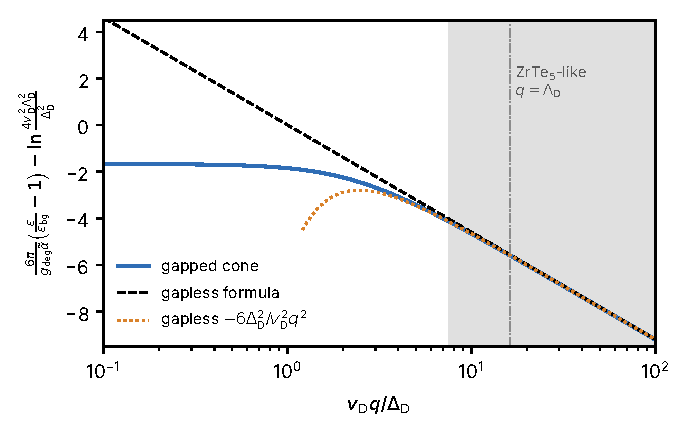
\includegraphics[width=\linewidth]{figures/ch07/limit7_gapless.pdf}
\captionof{figure}{Static dielectric function of a gapped Dirac cone against the gapless formula. Plotted is the induced part $\varepsilon(q,0)/\varepsilon_{\mathrm{bg}} - 1$ in units of $g_{\mathrm{deg}}\tilde\alpha/6\pi$, less the cutoff term $\ln(4v_{\mathrm{D}}^2\Lambda_{\mathrm{D}}^2/\Delta_{\mathrm{D}}^2)$, which makes the curves independent of the cutoff (hard cutoff on $|\vect{k}|$). Solid: \cref{eq:7.3-eps} at $\omega = 0$; dashed: the gapless formula, $-2\ln(v_{\mathrm{D}}q/\Delta_{\mathrm{D}})$ on this scale; dotted: the gapless formula with its leading correction $-6\Delta_{\mathrm{D}}^2/v_{\mathrm{D}}^2q^2$. Gray: $v_{\mathrm{D}}q > 7.5\,\Delta_{\mathrm{D}}$, where the gapless formula is within 0.1 of the full result; with the correction this holds from $3.7\,\Delta_{\mathrm{D}}$, and at $v_{\mathrm{D}}q = 10\,\Delta_{\mathrm{D}}$ the residual is $3\times10^{-3}$. Dash-dotted: $q = \Lambda_{\mathrm{D}}$ for the ZrTe$_5$-like cone of \cref{we:7-zrte5}, where $v_{\mathrm{D}}\Lambda_{\mathrm{D}} = 16.2\,\Delta_{\mathrm{D}}$. The Dirac region ends there.}\label{fig:7-gapless-limit}
\par}
\smallskip
Below $v_{\mathrm{D}}q \approx 2\Delta_{\mathrm{D}}$ the gapless formula diverges logarithmically, while the gapped cone saturates at \cref{eq:7.3-static}: the gap cuts off the pairs that would screen at long wavelength.
\end{limitbox}
The gapless formula follows from \cref{eq:7.3-eps} by expanding the logarithm for $|s| \gg \Delta_{\mathrm{D}}^2$: $\ln[1 - x(1 - x)s/\Delta_{\mathrm{D}}^2] \to \ln[-x(1 - x)s/\Delta_{\mathrm{D}}^2] + \Delta_{\mathrm{D}}^2/[-x(1 - x)s]$, and with $\int_0^1x(1 - x)\ln[x(1 - x)]\,\dd x = -5/18$ the constants $-\frac53$ cancel and $\Delta_{\mathrm{D}}$ drops out of the logarithm (\cref{eq:D.22-gapless}). The next term contributes $-6\Delta_{\mathrm{D}}^2/(v_{\mathrm{D}}^2q^2 - \omega^2)$ to the bracket. Static screening in a gapless cone, $\varepsilon(q,0) = \varepsilon_{\mathrm{bg}}[1 + (g_{\mathrm{deg}}\tilde\alpha/3\pi)\ln(2\Lambda_{\mathrm{D}}/q)]$, grows without bound as $q \to 0$, but only logarithmically. There is no screening length, since the density of states vanishes at the node; the electron gas screens a charge completely beyond $1/k_{\mathrm{TF}}$, whereas a gapless Dirac material only reduces it by a slowly growing factor.

The logarithms also set the validity of the calculation. The random-phase approximation keeps the first term in $\tilde\alpha$ of the polarization, and the induced part of \cref{eq:7.3-eps} is of order $g_{\mathrm{deg}}\tilde\alpha\ln(v_{\mathrm{D}}\Lambda_{\mathrm{D}}/\max(\Delta_{\mathrm{D}}, v_{\mathrm{D}}q))$, up to the numerical factor $1/3\pi$. We take this product as the expansion parameter: perturbation theory is reliable when it is small compared with one. Reading the screened interaction $e^2/\varepsilon q^2$ as a coupling that depends on $q$, the screening makes it weaker at smaller $q$, the counterpart of the running of the fine-structure constant in quantum electrodynamics, and the theory becomes weakly coupled at long wavelength~\cite{hochberg2018detection}. For $\tilde\alpha \gtrsim 1$ the one-loop result is an estimate, and what replaces it is an open question that \cref{sec:16.1} takes up.

Anisotropy enters through a rescaling. With $\delta k_i \to \delta k_i/v_i$, the Hamiltonian \cref{eq:7.3-H} becomes isotropic with unit velocity, the sum over $\vect{k}$ acquires the Jacobian $1/(v_1v_2v_3)$, and $q^2$ in the overlap becomes $\sum_iv_i^2q_i^2$ (\cref{app:D.22}). The cutoff becomes an ellipsoid in $\vect{k}$, a sphere of radius $\Lambda_{\mathrm{D}}v_{\mathrm{D}}$ in energy units for the rescaled momenta. For $\vect{q}$ along the principal axis $i$, the Coulomb factor $e^2/q^2$ then multiplies $v_i^2/(v_1v_2v_3)$ in place of $1/v_{\mathrm{D}}$, and the background constant becomes its component $\varepsilon_{\mathrm{bg},ii}$ along that axis, assuming the background and the cone share principal axes. The static constant along $i$ is
\begin{equation}
  \varepsilon_{ii}(0,0) = \varepsilon_{\mathrm{bg},ii} + \frac{g_{\mathrm{deg}}\alpha}{3\pi}\,\frac{v_i^2}{v_1v_2v_3}\Bigl(\ln\frac{2\tilde\Lambda}{\Delta_{\mathrm{D}}} - \frac56\Bigr) ,
  \label{eq:7.3-aniso}
\end{equation}
with $\tilde\Lambda$ the cutoff on the energy $(\sum_iv_i^2\delta k_i^2)^{1/2}$. Along each axis the effective coupling is $\alpha v_i^2/(\varepsilon_{\mathrm{bg},ii}v_1v_2v_3)$, which reduces to \cref{eq:7.3-alpha} for an isotropic cone.

The four inputs of \cref{eq:7.3-eps}, $v_i$, $\Delta_{\mathrm{D}}$, $\Lambda_{\mathrm{D}}$ and $\varepsilon_{\mathrm{bg}}$, come from first-principles calculations. The velocities and the cutoff are fitted to a computed band structure near the node (\cref{app:E.1}). The half-gap is the delicate one: semilocal functionals misplace small gaps and can invert the band order, and quasiparticle corrections (\cref{app:E.3}) or the measured gap are needed. The background constant comes from density-functional perturbation theory (\cref{app:E.4}) or from the random-phase sum over bands (\cref{app:E.6}). Both compute the dielectric constant of the whole crystal, which includes the Dirac pairs, and they do so at the calculated gap, to which the Dirac term is sensitive through $\ln(1/\Delta_{\mathrm{D}})$. A consistent $\varepsilon_{\mathrm{bg}}$ leaves the Dirac bands out of the sum over transitions, or subtracts \cref{eq:7.3-static} from the computed total. The parameters of ZrTe$_5$ used in rate calculations are specified in \cref{app:E.20}.

\begin{workedexample}{Effective coupling and static screening of ZrTe$_5$}\label{we:7-zrte5}
ZrTe$_5$ has one gapped cone at $\mathrm{\Gamma}$, $g_{\mathrm{deg}} = 2$. We take the first-principles values for the measured crystal structure~\cite[Table~1 and text below it]{geilhufe2020dirac}. They are the principal velocities $v_x, v_y, v_z = 1.1\times10^{-3}$, $4.5\times10^{-4}$, $1.0\times10^{-3}$, a gap of \SI{23.6}{meV} ($\Delta_{\mathrm{D}} = \SI{11.8}{meV}$), and cutoffs $\Lambda_x, \Lambda_y, \Lambda_z = 0.23$, $0.215$, \SI{0.1}{\angstrom^{-1}}. A relaxed cell volume gives the same $v_x$, slower $v_y = 4.4\times10^{-4}$ and $v_z = 9.1\times10^{-4}$, and a gap of \SI{31.2}{meV} ($\Delta_{\mathrm{D}} = \SI{15.6}{meV}$); the reference implements that row in its rates. The dielectric tensor from density-functional perturbation theory has the diagonal components 308.4, 20.75 and 126.1~\cite[Table~2]{geilhufe2020dirac}.

\emph{Cutoff.} With $\SI{1}{\angstrom^{-1}} = \SI{1.973}{keV}$, the band energies at the three cutoffs are $v_i\Lambda_i = 0.499$, $0.191$ and \SI{0.197}{eV}. The cone is linear to a much higher energy along $x$ than along $y$. We keep the states with $(\sum_iv_i^2\delta k_i^2)^{1/2} < \tilde\Lambda = \SI{0.191}{eV}$, the smallest of the three~\cite[Eq.~(2.21)]{geilhufe2020dirac}, a conservative choice that a better fit of the bands would replace by a larger ellipsoid. Their dielectric function, Ref.~\cite[Eq.~(3.10)]{geilhufe2020dirac}, carries the same constant $-\frac53$ as \cref{eq:7.3-eps}, so that $\tilde\Lambda$ is a hard cutoff in our sense, $\tilde\Lambda = v_{\mathrm{D}}\Lambda_{\mathrm{D}}$.

\emph{Isotropic estimate.} To get a single number, replace the cone by an isotropic one with the same density of states, $v_{\mathrm{D}} = (v_xv_yv_z)^{1/3} = 7.9\times10^{-4}$, and the tensor by the harmonic mean of its components, $\varepsilon_{\mathrm{bg}} = 3/(\sum_i1/\varepsilon_{\mathrm{bg},ii}) = 50.5$, the average used in Ref.~\cite{hochberg2018detection}. Then \cref{eq:7.3-alpha} gives $\tilde\alpha = 0.18$ and $g_{\mathrm{deg}}\tilde\alpha = 0.37$. The cutoff in momentum is $\Lambda_{\mathrm{D}} = \tilde\Lambda/v_{\mathrm{D}} = \SI{241}{eV} = \SI{0.12}{\angstrom^{-1}}$. An earlier calculation~\cite[Table~1]{hochberg2018detection}, with faster velocities ($2.9\times10^{-3}$, $5.0\times10^{-4}$, $2.1\times10^{-3}$) and smaller dielectric constants (187.5, 9.8 and 90.9, harmonic mean 25.3), yields a similar $\tilde\alpha = 0.20$, quoted there as $g_{\mathrm{deg}}\tilde\alpha = 0.80$ with $g_{\mathrm{deg}} = 4$ states per band.

\emph{Static screening.} With $\ln(2\tilde\Lambda/\Delta_{\mathrm{D}}) = \ln 32.4 = 3.48$, \cref{eq:7.3-static} yields
\begin{equation*}
  \frac{\varepsilon(0,0)}{\varepsilon_{\mathrm{bg}}} - 1 = \frac{0.37}{3\pi}\,(3.48 - 0.83) = 0.102 ,
\end{equation*}
so that $\varepsilon(0,0) = 55.7$. The Dirac electrons add \SI{10}{\percent} to the screening of the background. At finite $q$, the integral in \cref{eq:7.3-eps} reduces this to 0.091 at $q = 2\Delta_{\mathrm{D}}/v_{\mathrm{D}} = \SI{30}{eV}$ and to 0.052 at $q = \Lambda_{\mathrm{D}}/2 = \SI{121}{eV}$, momenta at which sub-MeV dark matter scatters (\cref{fig:7-dirac}b). The expansion parameter at long wavelength, $g_{\mathrm{deg}}\tilde\alpha\ln(v_{\mathrm{D}}\Lambda_{\mathrm{D}}/\Delta_{\mathrm{D}}) = 0.37\ln 16.2 = 1.0$, is about one. The induced term itself, 0.102, is small mainly through the factor $1/3\pi$, and the one-loop result is a fair estimate of it. Since $v_{\mathrm{D}}\Lambda_{\mathrm{D}} = 16.2\,\Delta_{\mathrm{D}}$, ZrTe$_5$ reaches the gapless regime of \cref{fig:7-gapless-limit} only above $v_{\mathrm{D}}q = 7.5\,\Delta_{\mathrm{D}}$, or $q = \SI{112}{eV}$: below that momentum the gap matters.

\emph{Anisotropy.} Along the principal axes, \cref{eq:7.3-aniso} with $\ln(2\tilde\Lambda/\Delta_{\mathrm{D}}) - \frac56 = 2.64$ adds 10.0, 1.67 and 8.3 to the background components 308.4, 20.75 and 126.1, that is 3.2, 8.1 and \SI{6.6}{\percent}. The effective couplings along the three axes, $\alpha v_i^2/(\varepsilon_{\mathrm{bg},ii}v_xv_yv_z)$, are 0.058, 0.144 and 0.117: the slow direction $y$ has the smallest background constant as well, and it is the most strongly coupled. The averaged $\tilde\alpha = 0.18$ is a fair summary, though it overstates the coupling along $x$ threefold.

\emph{Size of the Dirac screening.} The Dirac contribution is 3 to \SI{8}{\percent} of the dielectric constant, smaller than the spread between the two sets of computed parameters. Both sets of dielectric constants are totals for the whole crystal, computed at a gap of 24 to \SI{35}{meV}, and already contain a Dirac term of this size, which is harmless at the few-percent level. The coupling that matters for a rate is the total $\varepsilon$, dominated here by the background: with $\varepsilon \approx 56$, every Coulomb-like interaction inside ZrTe$_5$ is reduced about fifty-fold.
\end{workedexample}

Dirac materials screen the interaction mostly through their large background dielectric constant, with the Dirac electrons adding a logarithm of order $g_{\mathrm{deg}}\tilde\alpha$. The loss function that follows from \cref{eq:7.3-eps}, and the rates of scattering and absorption with the background placed in the total $\varepsilon$ as in \cref{eq:7.3-epsbg}, are the subject of \cref{sec:16.1}.
